\subsubsection{Board Representation}

Since the computer cannot work with a physical chess board and pieces, these must be converted into a form in which the board, pieces, and position can be interpreted by the computer and later used for the input layer of the neural network. The most common way of representing positions and movements of chess pieces is the data structure bitboards. A bitboard is implemented as an $8 \times 8$ bit array, which is the size of a chessboard.\footnote{Cf. \cite{boskovic-2005-bb}, p. 360} Each array element corresponds to a square on the board. A bitboard is created for each type of piece (pawn, knight, bishop, rook, queen and king) of a given color (black and white). Further 4 board for "2 casteling choices of each player"\footnote{\cite{zang-etal-2019-automated}} are generated. This gives a total number of 16 bitboards. Finally, the squares on which the figures are placed must be marked on the respective boards. This can be done in binary, where 0 means the square is empty and 1 means the square is not empty.

\begin{figure}[h]
\centering
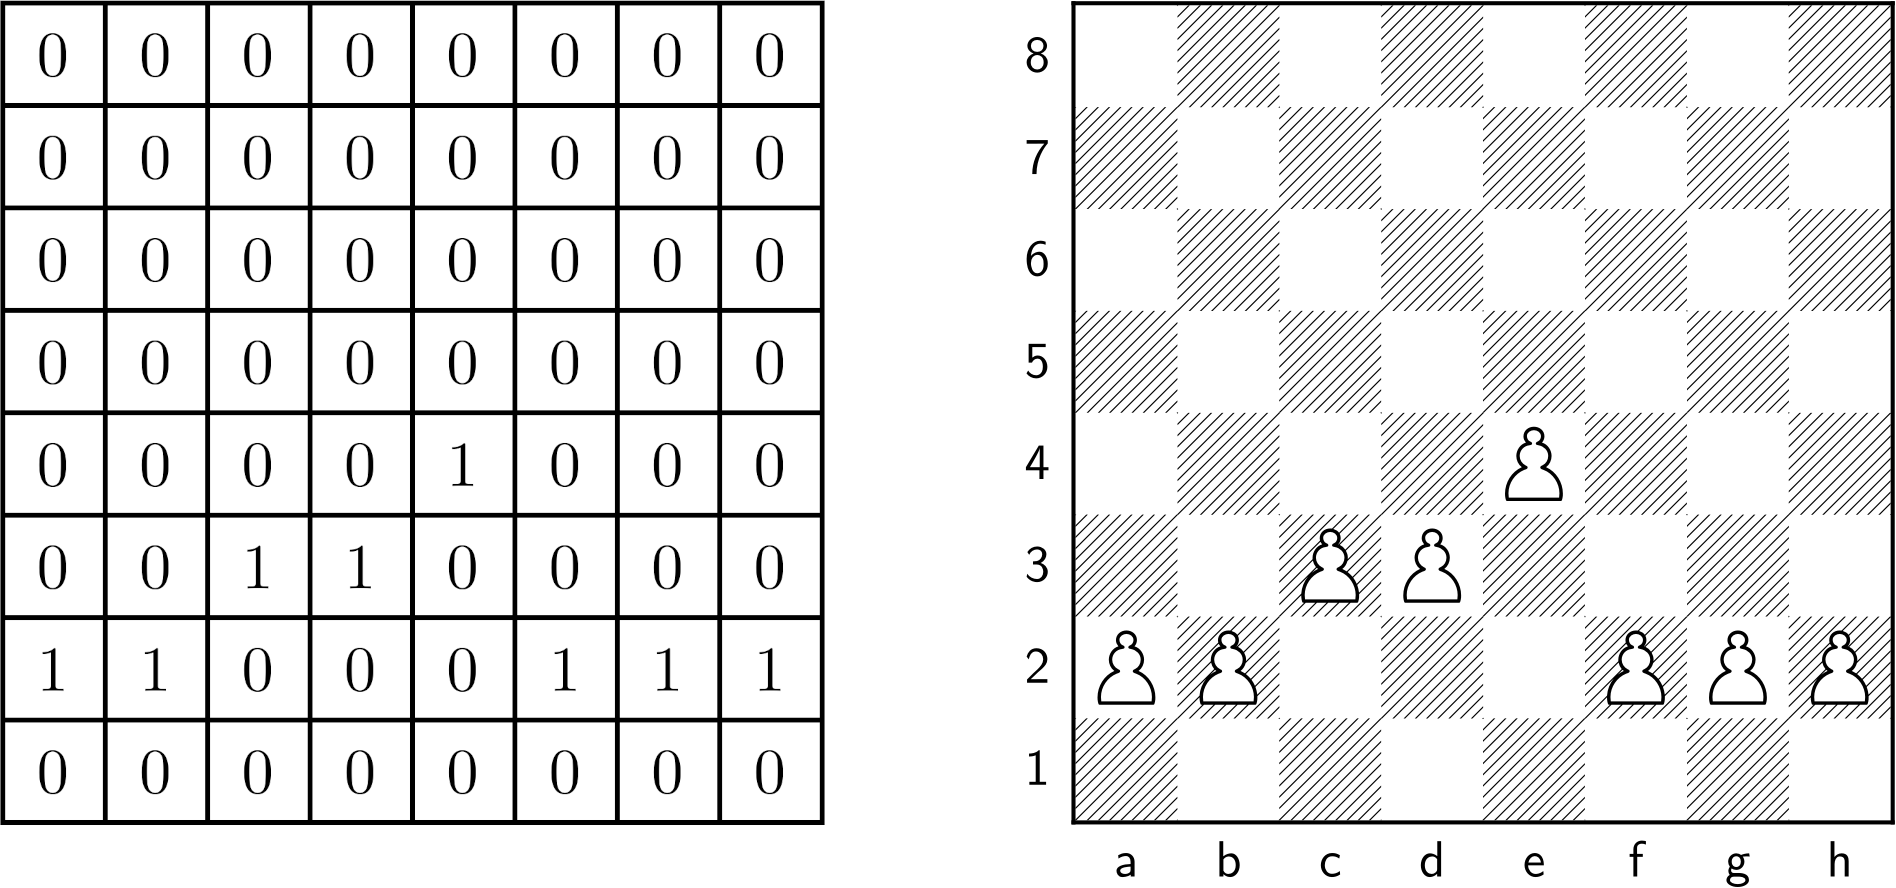
\includegraphics[width=0.5\textwidth]{graphics/bitboard/bitboard_and_chessboard.png}
\caption{Representation of bitboard with white pawns (left) and the corresponding chessboard (right)}
\end{figure}

Bitboards can also be used to represent possible movements of chess pieces. This is achieved by performing certain logical operations on the bitboard. The main advantage of the logical operations are, that they can be executed quite quickly by the processor.\footnote{Cf. \cite{boskovic-2005-bb}, p. 360} Furthermore, with x64 processors the position can be stored in a bit string in the memory, since this is exactly 64 bits long due to the number of squares.\footnote{Cf. \cite{segundo-2005-bb}, p. 67} Another advantage is that it can be used as input for the input layer in the neural network due to its simple representation. The network could then be trained to evaluate specific chess positions and predict moves.